\documentclass{article}
\usepackage{array, tabularx}

\usepackage{graphicx}

\usepackage{pdfpages}
\newcolumntype{Y}{>{\centering\arraybackslash}X}

\newdimen\demilargeur
\demilargeur=\textwidth
\divide\demilargeur by 2
\newcommand\tab[1][1cm]{\hspace*{#1}}
\begin{document}
\title{Protocole de communication graphique 2D}
\date{}
\author{Fatima-Ezzohra AKHTEN et Arthur DELAIN}
\maketitle
\begin{abstract}
\begin{center}
Réseaux, L3 Informatique UCA Clermont-Ferrand,2019\\
\end{center}
\end{abstract}
\part*{Introduction}
Vous avez sûrement déjà remarqué des pictogrammes fait de petits carrés noirs et blancs que ce soit sur des affichages publicitaires, sur un e-billet, sur l’emballage des produits de consommation, ou même dans un magazine, et vous vous êtes demandé de quoi s’agit-il? En effet, c’est un code 2D appelé plus généralement Tags, QR Codes ou Flashcodes; l'héritier du code barre à une dimension mais ayant une technologie plus avancée.\\

Les codes 2D permettent de passer d'un support physique (papier, écran…) au format électronique en une fraction de seconde, dans le but de traiter ou capturer des données (URL, mail, carte de visite…).\\

Ils se caractérisent par le fait qu'ils contiennent des informations à la fois verticalement et horizontalement. Par conséquent les codes barres 2D contiennent beaucoup plus d'informations (stockées dans une matrice 2D) qu'un code barre classique à une dimension.\\

 
Le format des codes à barres 2D est généralement issu de deux technologies d'encodage : datamatrix et QR Code. Ces technologies d'encodage permettent de stocker une grande quantité d'information sur un espace réduit en comparaison des codes à barres à une seule dimension. \\

Pour notre projet, on s'est basé sur la deuxième technologie d'encodage qu'est le QR Code, dont le format est direct, qui permet de contenir directement un grand nombre de données dans le code, et qui peut être décodé rapidement.


\part*{Sujet}
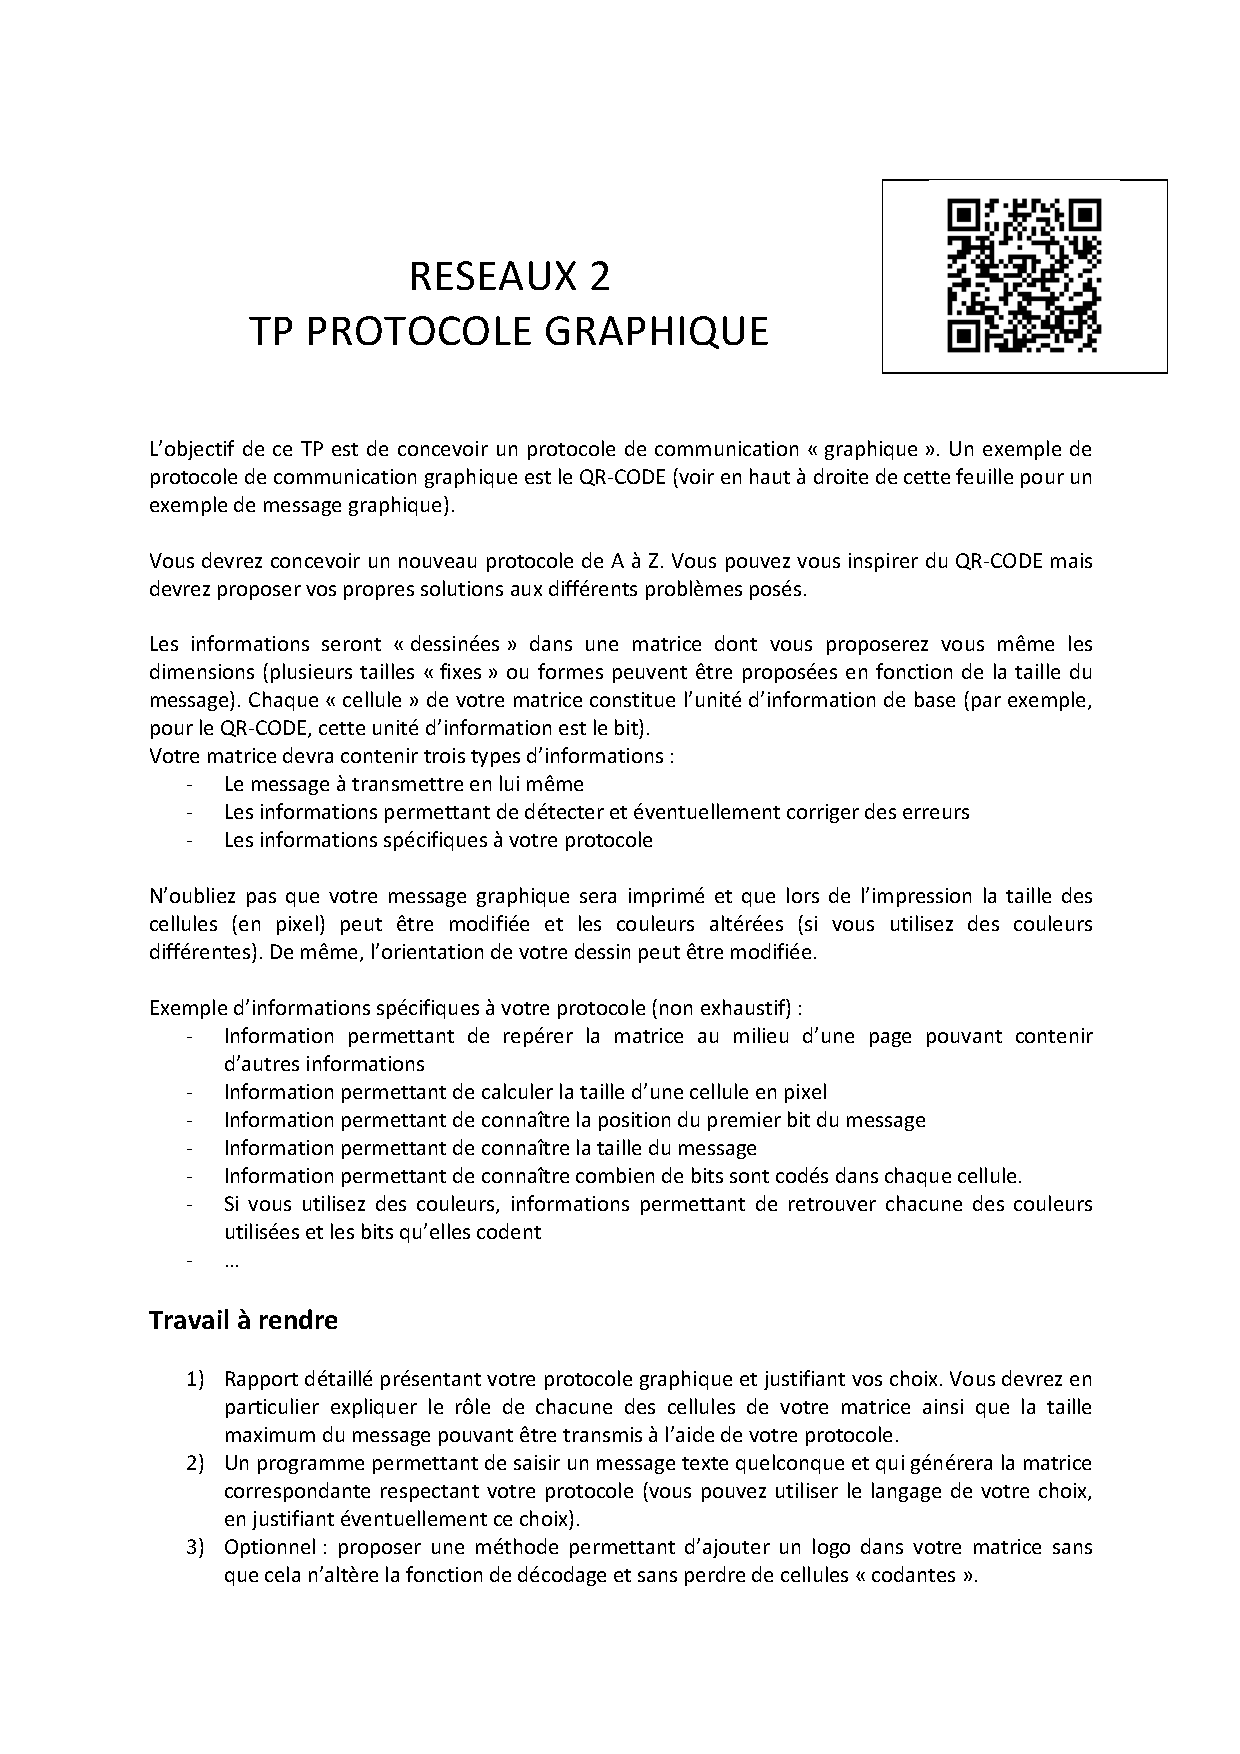
\includepdf[scale=0.80]{TPReseaux2.pdf}
\part{Fonctionnement}

$\bullet$ 1 - Tout d'abord, il faut analyser les données à encoder et paramétrer le niveau de code correcteur (expliqué plus loin).
Cela permet d'analyser les entrées afin d'obtenir la variété des caractère à encoder. 
\\ \\
$\bullet$ 2 - Il faut ensuite convertir les données dans un flux de bytes.\\
\\
Les premier bits d'information represente souvent le mode (alpha numeric,...).
Il faut donc encoder les données et les concaténer entre elles avec le code correcteur 
Par exemple le mode QrCode est sur 4bits :\\\\
\begin{tabularx}{\linewidth}{|Y|Y|Y|}
\hline
Indicateur binaire & Type charactère \\\hline
0001  &	Numérique\\
0010  &	Alphanumérique\\
0100  &	Binaire\\
1000  &	Kanji (caractère Japonais)\\
\hline
\end{tabularx}\\\\
(non exhaustif)\\
On peut ensuite mettre en place après l'avoir choisi le niveau de correction du code de correction d'erreur afin de créer une structure de messages finale (block de bits)\\\\
Et ensuite on peut creer les différents ajout complémentaire:\\
Il faut indiquer la version (si il y en a plusieurs taille de Code 2D), le format , taille du message , ...\\\\
\\
$\bullet$ 3 - On implémente de la verification et correction des erreurs.
On sépare le message en bits en blocs de bits de données et on genère le codes correcteurs.\\
Le code correcteur le plus répandu est Redd-Salomon, il peut avoir différents niveau :\\
\\
\begin{tabularx}{\linewidth}{|Y|Y|Y|}
\hline
Niveau & Redondance & Indicateur binaire \\\hline
L & environ 7 \% & 01\\
M & environ 15 \% & 00\\
Q & environ 25 \% & 11\\
H & environ 30 \% & 10 \\
\hline
\end{tabularx}\\\\
L'illustration la plus courante de ça mise en place sur internet est celle ci :\\
\begin{center}
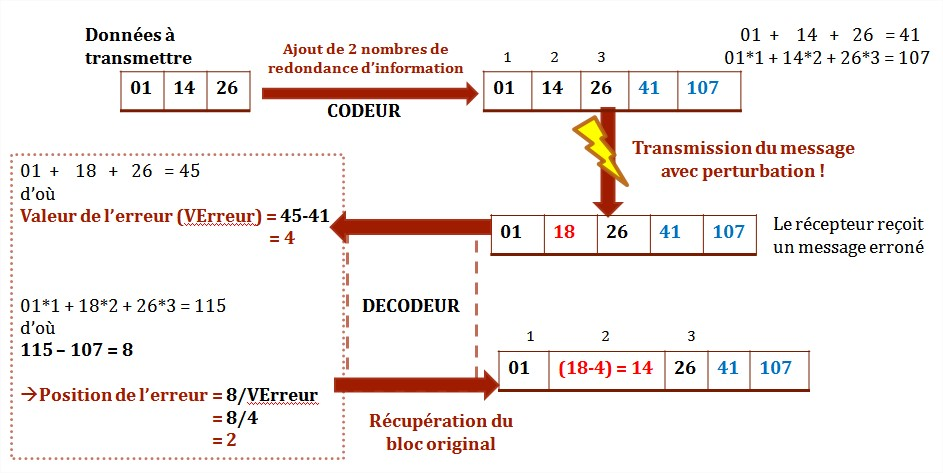
\includegraphics[scale=0.4]{detectcorrect.jpg} 
\end{center}
(Il y a aussi le Code de Hamming et d'autres moins connus)
Si il n'y a pas de niveau de code correcteur spécifié, pour le Qr Code par exemple la plus petite version de celui ci est utilisée.\\
Il y a bien sur différents codes correcteurs et manière de vérifier les informations. Par exemple on peut générer un hashcode du message et l’intégrer dans celui pour que lors du scan du Code 2D l'on puisse savoir directement si le message n'a pas été corrompu.\\
\\
$\bullet$ 4 - On insère ensuite les données avec le code correcteur une matrice.\\    
On peut ensuite placer les différents éléments:\\
$\tab\rightarrow$ les motifs de positionnement qui sont des séparateurs afin distinguer les differents éléments ainsi que de reperer le Code 2D dans un document.\\
$\tab\rightarrow$ les motifs de synchonisation/Timming patterns permettant de percevoir les contrastes entre les modules (clairs et foncés) et il permettent de determiner la version du Qr code (avec ça taille.)\\
$\tab\rightarrow$ les motifs de d'alignement qui sont pareil mais plus petit que les motifs de positionnement, il servent dans le cas ou il ya des versions très grande du Code 2D, cela facilite la lecture en cas de deformation de la matrice.\\
$\tab\rightarrow$ zone tranquille autour du symbol/matrice. Il s-agit de zone vide afin de bien d'elimiter les differents elements.\\
$\tab\rightarrow$Placement le message en bits (avec ses informations complémentaires).\\
\\
(voir schema Qr Code pour exemple)
\\\\\\
$\bullet$ 5 - On génère la matrice et l'évaluation du résultat retourné.\\
Afin d'avoir une bonne repartition des élements dans le code 2d on utilise des masques de patterns. 
Cela permet d'optimiser la balance entre les modules noirs et les modules blancs (cela améliore donc la répartition) et aussi de minimiser les occurrences de patterns indésirables \\
	$\tab$On creer donc différents masques à appliquer et on applique celui/ceux juger le meilleurs (note donné à chaque masque)\\
	$\tab$Application du masque\\
Exemple du QR code :\\
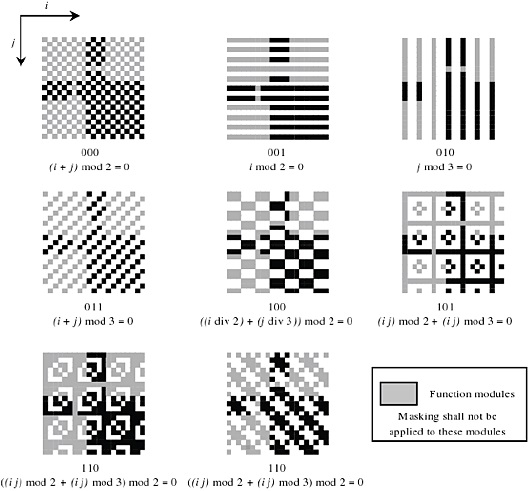
\includegraphics[scale=1]{qrcode-masque.jpg} 
\\ \\
On peut ensuite intégrer les differentes information de format et de version à des endroits spécifique.
Exemple du QR code:\\
\begin{center}
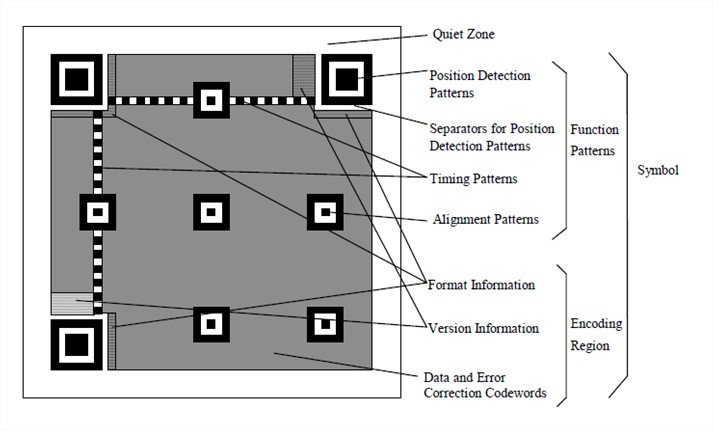
\includegraphics[scale=0.65]{qrmainstruct.jpg} 
\end{center}
$\bullet$ 6 - Génération du Code 2D au format image.\\
\\
(lecture\\
    $\tab$1 - Reconnaître les bits 1 ou 0.\\
    $\tab$2 - Identifier le taux de code correcteur (avec masque -> format).\\
    $\tab$3 - Identifier la version/format du Code.\\
    $\tab$4 - Découvrir région à décoder.\\
    $\tab$5 - Lire les données et le code correcteur.\\
    $\tab$6 - Détecter/Corriger les erreurs.\\
    $\tab$7 - Décoder données.\\
    $\tab$8 - résultat.\\
)\\
\\
On peut prendre comme exemple  un logiciel open source de générateur de Qr Code ZXing, ecrit en java.\\

\part{Mise en place}
Le langage uilisé dans notre projet est le java, avec swing pour générer une interface graphique. Le logiciel est développé sous l'IDE Intel ij.

Le nom de notre Code 2D est Code Fort par son allure en carré "concentrique" rappelant une muraille avec un donjon comme zone d'inclusion  
\subsection{Encodage et versionnage:}
Versionnage :
Apres avoir définit un versionnnage se voulant proportionnel à la taille du message à encoder nous avons décider pour des raisons de simplicité de le laisser fixe à 32x32 cases pour le message en bits en lui même. (Il n'est donc pas necessaire de l'indiquer, mais celui ci pourra etre ajouter au information de format (8 bit pr le format et 8 bit pour la version et 8 bits pour la taille)) \\
\\
Ecodage:
Nous avons choisi comme encodage le bit avec un pixel blanc pour le 0 et un noir pour le 1 (traduit en tableau de Boolean dans le code). Les élements sont défini selon leur Code ASCII. Il seront dont encodé sur 8 bits (lettres, nombres et charactères speciaux)
Notre Version seul peut donc encoder un maximum de 128 caractères. (Cela sans indication d'encodage pouvant par la suite être integré) 
\\\\\\
\begin{center}
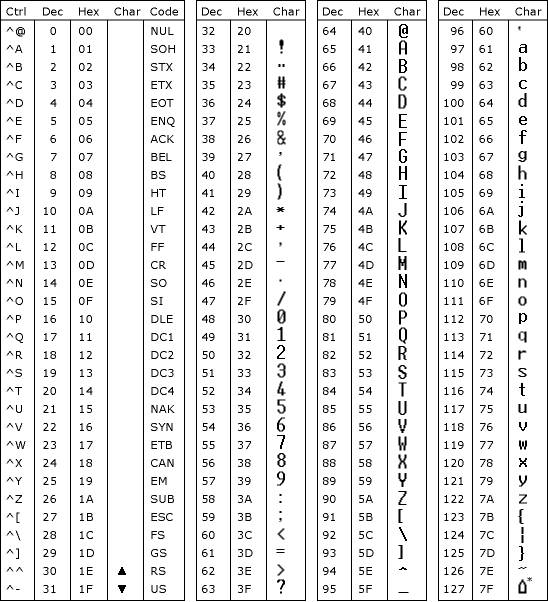
\includegraphics[scale=0.5]{code_ascii_1.jpg} 
\end{center}
\subsection{Code correcteur:}
Apres avoir commencer de créer un systeme de correction d'erreur avec Redd Salomon, la tache fut simplifié en intégrant seulement un hashcode des donnéees générées cela afin lors de la lecture de verifier l'intégrité du message. (le hashcode nouvelement créé avec le message scanné est comparé à l'ancien hashcode indiqué en début de message et dont la taille est pour notre projet de 32bits (norme java))
\\
\subsection{Insertion (les differents motifs):}
Un pemier contour au message encodé est créé afin de faire une zone tranquille/tampon autour de celui-ci. Et afin de séparer le message des autres informations indiqué (version dans le cas future ou l'on en rajouterai, format,...). Ce dernier sera lui même entouré d'un contour (double pixel : blanc puis noir) servant de pattern de positionnement.\\
C'est l'alterance entre ces différents contour permet de calculer la taille d'un pixel
\\
\subsection{ generation matrice ( masque,format,version) :}
On peut ensuite rajouter les différentes informations complémentaires dans la zone entre le contour exterieur et le contour du message.\\
taille information complementaire : 32 bits -> 4 bits pour le masque, 4 bits code correcteur, 8 bits pour la taille du message, 8 bits pour le format et 8 bits pour la version.
On applique ensuite un masque (choisi par default ici, il aurait fallu caluler celui ayant la meilleur répartion vis à vis des autres).
\\
\subsection{Generation Code 2D:}
Après avoir optenu une matrix de 0 et de 1 (utilisation du Boolean[][]) on peut directement générer le Code 2D Graphique correspondant en plaçant des pixels noirs aux emplacements des 1 (comme dit precedemment).
\\\\
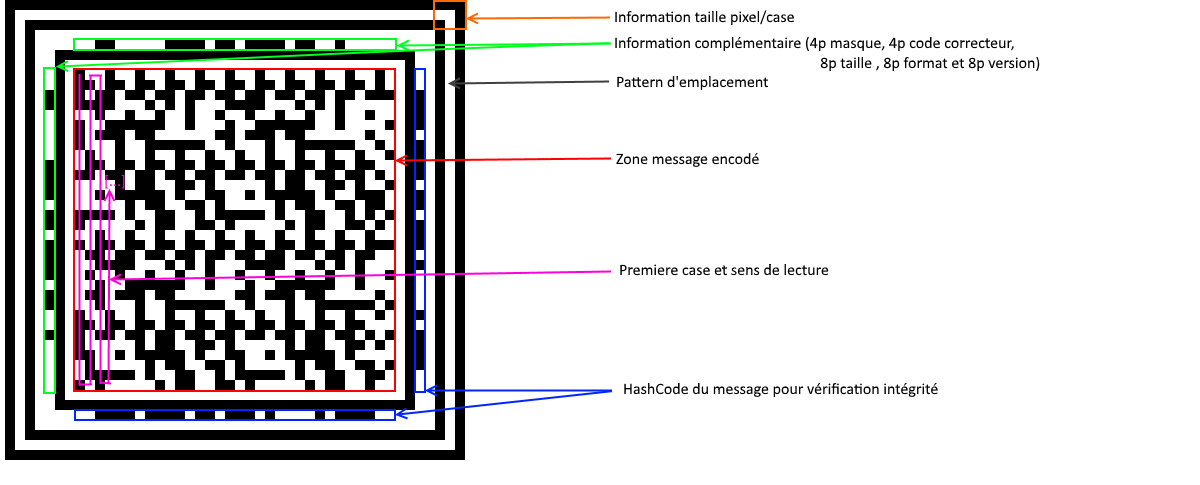
\includegraphics[scale=0.5]{schema2.png} 
\\\\

\part{Utilisation}
Lancer le .jar (avec java) placé dans la racine du projet:\\
Etapes:\\
$\tab$1) rentrer le texte dans la fentre pop-up \\
\begin{center}
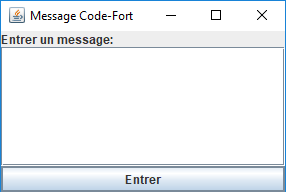
\includegraphics[scale=1]{exemple_text.png} 
\end{center}
$\tab$2) generer l'image correspondante (bouton Entrer de la fenetre pop up)
\begin{center}
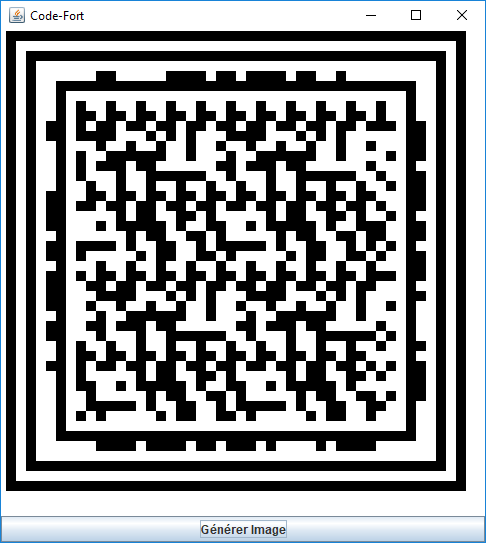
\includegraphics[scale=0.5]{exemple.png}
\end{center}
$\tab$2) enregistrer l'image (bouton correspondant)
\begin{center}
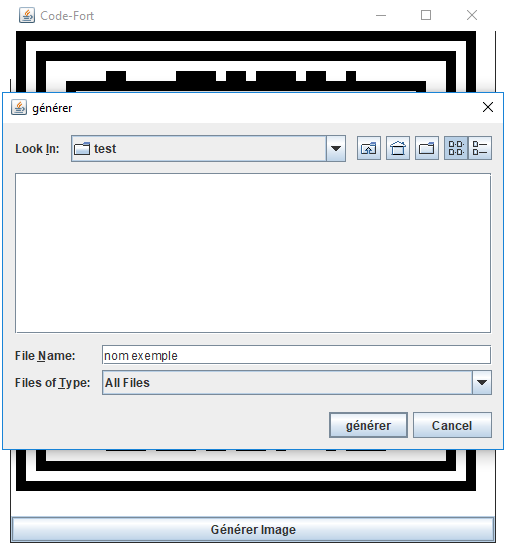
\includegraphics[scale=0.5]{exemple_generation.png} 
\end{center}
\end{document}